\documentclass{article}
\usepackage{tikz}
\usepackage[left=0.15cm, right=2cm, top=0.5cm, bottom=0.5cm]{geometry}
\usepackage{xcolor}
\usepackage{setspace}

% Definir colores personalizados
\definecolor{lightyellow}{HTML}{FFF9C4}
\definecolor{softpeach}{HTML}{FFE0B2}
\definecolor{palegreen}{HTML}{DCEDC8}
\definecolor{skyblue}{HTML}{BBDEFB}
\definecolor{lavender}{HTML}{E1BEE7}
\definecolor{mint}{HTML}{B2DFDB}
\definecolor{lightgray}{HTML}{F5F5F5}
\definecolor{pastelpink}{HTML}{F8BBD0}
\definecolor{powderblue}{HTML}{B3E5FC}
\definecolor{lemoncream}{HTML}{FFF8E1}


\begin{document}

\begin{footnotesize}
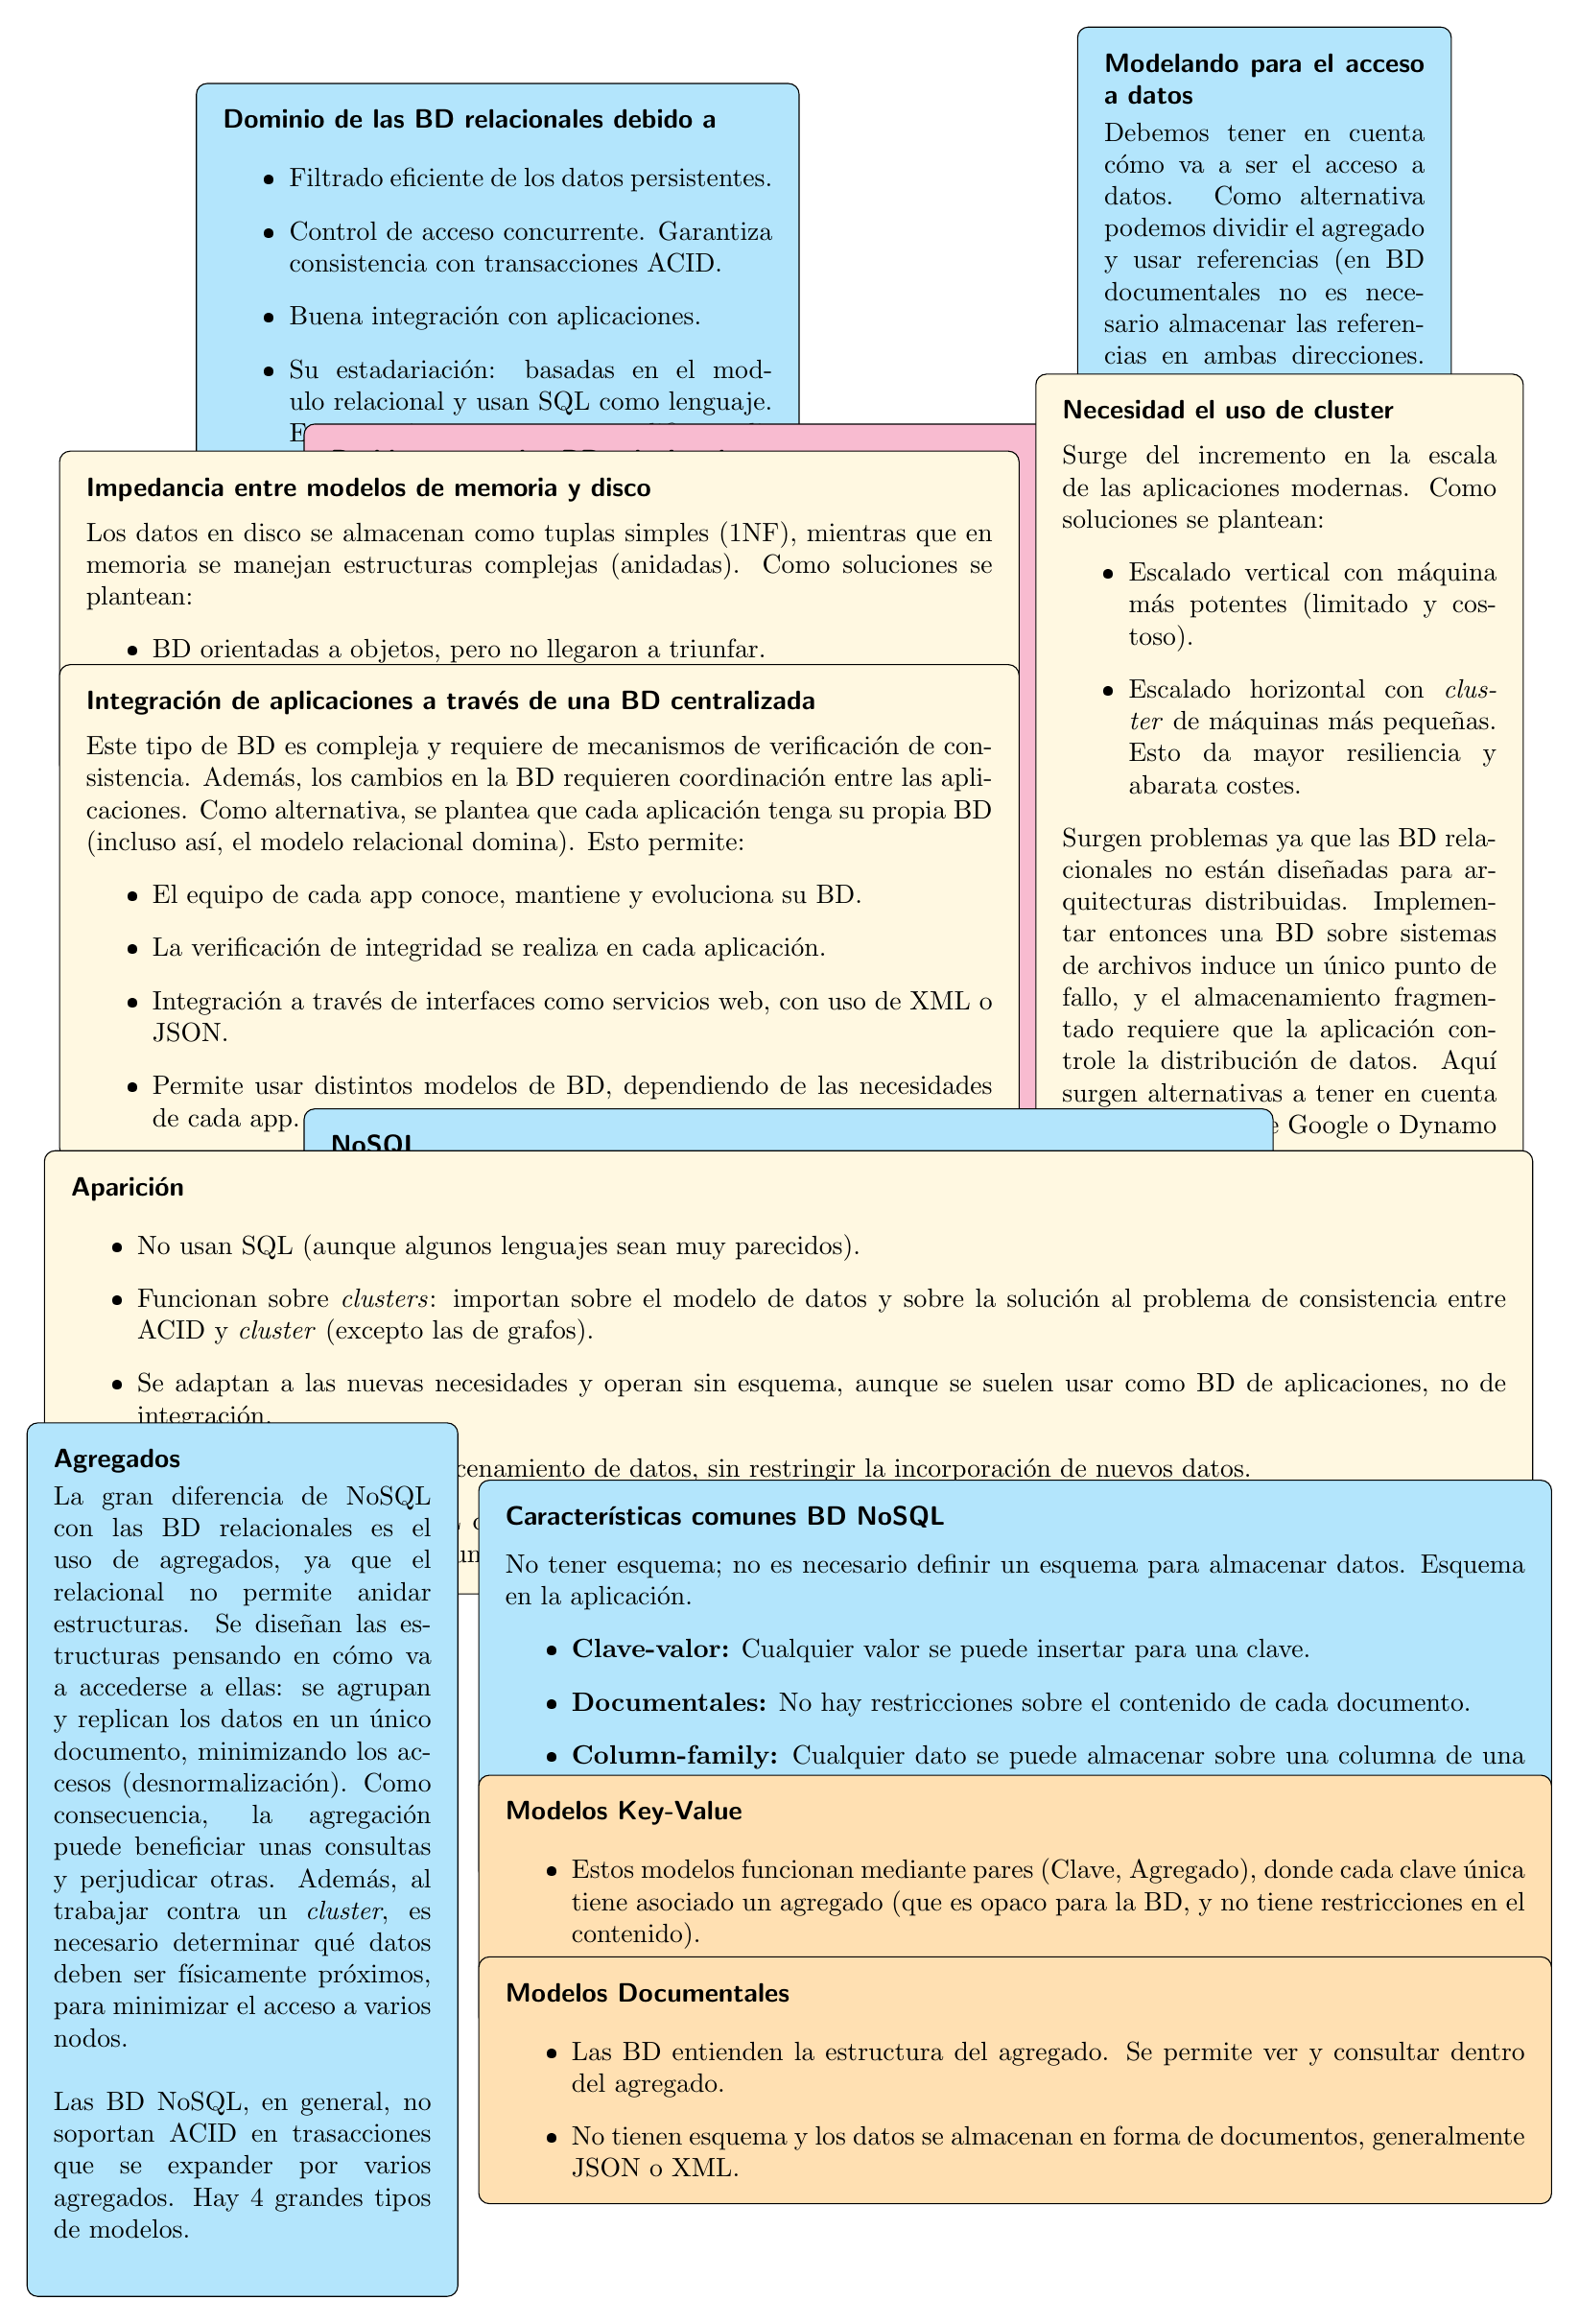
\begin{tikzpicture}
    \node[fill=powderblue, fill opacity=1, text opacity=1, text width=0.6\textwidth, align=justify, draw, rounded corners, inner sep=10pt] 
    (note1) at (-3.85, 0) {
        \textbf{\textsf{Dominio de las BD relacionales debido a }} \\[-10pt]
        \begin{itemize}
        \item Filtrado eficiente de los datos persistentes.
        \item Control de acceso concurrente. Garantiza consistencia con transacciones ACID. 
        \item Buena integración con aplicaciones.
        \item Su estadariación: basadas en el modulo relacional y usan SQL como lenguaje. Esto permite no tener que recodificar aplicaciones al cambiar la BD.
        \end{itemize}
    };

    \node[fill=powderblue, fill opacity=1, text opacity=1, text width=0.35\textwidth, align=justify, draw, rounded corners, inner sep=10pt] 
    (note1) at (6.3, 0) {
        \textbf{\textsf{Modelando para el acceso a datos}} \\[2pt]
        Debemos tener en cuenta cómo va a ser el acceso a datos. Como alternativa podemos dividir el agregado y usar referencias (en BD documentales no es necesario almacenar las referencias en ambas direcciones. Debemos calcular el agregado para hacer consultas analícas (excepto en documentales, pero no es eficiente). 
    };

    \node[fill=pastelpink, fill opacity=1, text opacity=1, text width=\textwidth, align=justify, draw, rounded corners, inner sep=10pt] 
    (note2) at (0, -6.3) {
        \textbf{\textsf{Problemas con las BD relacionales}} \\[220pt]
    };

    \node[fill=lemoncream, fill opacity=1, text opacity=1, text width=12cm, align=justify, draw, rounded corners, inner sep=10pt] 
    (note2) at (-3.3, -4.25) {
        \textbf{\textsf{Impedancia entre modelos de memoria y disco}} \\[5pt]
        Los datos en disco se almacenan como tuplas simples (1NF), mientras que en memoria se manejan estructuras complejas (anidadas). Como soluciones se plantean:
        \begin{itemize}
        \item BD orientadas a objetos, pero no llegaron a triunfar.
        \item El mapeado objeto-relacional no resuleve el problema del todo, pero induce nuevos problemas, como la ineficiencia al evitar el uso del SGBD.
        \end{itemize}
    };

    \node[fill=lemoncream, fill opacity=1, text opacity=1, text width=12cm, align=justify, draw, rounded corners, inner sep=10pt] 
    (note2) at (-3.3, -8.2) {
        \textbf{\textsf{Integración de aplicaciones a través de una BD centralizada}} \\[5pt]
        Este tipo de BD es compleja y requiere de mecanismos de verificación de consistencia. Además, los cambios en la BD requieren coordinación entre las aplicaciones. Como alternativa, se plantea que cada aplicación tenga su propia BD (incluso así, el modelo relacional domina). Esto permite:
        \begin{itemize}
        \item El equipo de cada app conoce, mantiene y evoluciona su BD.
        \item La verificación de integridad se realiza en cada aplicación.
        \item Integración a través de interfaces como servicios web, con uso de XML o JSON.
        \item Permite usar distintos modelos de BD, dependiendo de las necesidades de cada app.
        \end{itemize}
    };

    \node[fill=lemoncream, fill opacity=1, text opacity=1, text width=5.75cm, align=justify, draw, rounded corners, inner sep=10pt] 
    (note2) at (6.5, -6.5) {
        \textbf{\textsf{Necesidad el uso de \textit{cluster}}} \\[5pt]
        Surge del incremento en la escala de las aplicaciones modernas. Como soluciones se plantean:
        \begin{itemize}
        \item Escalado vertical con máquina más potentes (limitado y costoso).
        \item Escalado horizontal con \textit{cluster} de máquinas más pequeñas. Esto da mayor resiliencia y abarata costes.
        \end{itemize}
        Surgen problemas ya que las BD relacionales no están diseñadas para arquitecturas distribuidas. Implementar entonces una BD sobre sistemas de archivos induce un único punto de fallo, y el almacenamiento fragmentado requiere que la aplicación controle la distribución de datos. Aquí surgen alternativas a tener en cuenta como Big Table de Google o Dynamo de Amazon.
    };
    \node[fill=powderblue, fill opacity=1, text opacity=1, text width=\textwidth, align=justify, draw, rounded corners, inner sep=10pt] 
    (note1) at (0, -13.8) {
        \textbf{\textsf{NoSQL}} \\ [2pt]
        No hay una definición clara del término. Inicialmente era ``BD no relaciones, distribuidas y de código abierto''.\\[105pt]
    };
    \node[fill=lemoncream, fill opacity=1, text opacity=1, text width=19cm, align=justify, draw, rounded corners, inner sep=10pt] 
    (note1) at (0, -14.3) {
        \textbf{\textsf{Aparición}} \\ [-10pt]
        \begin{itemize}
        \item No usan SQL (aunque algunos lenguajes sean muy parecidos).
        \item Funcionan sobre \textit{clusters}: importan sobre el modelo de datos y sobre la solución al problema de consistencia entre ACID y \textit{cluster} (excepto las de grafos).
        \item Se adaptan a las nuevas necesidades y operan sin esquema, aunque se suelen usar como BD de aplicaciones, no de integración. 
        \item Abre opciones para el almacenamiento de datos, sin restringir la incorporación de nuevos datos. 
        \item Hay que considerar NoSQL cuando el tamaño y rendimiento hagan necesarios el uso de un \textit{cluster} y por temas de productividad, ya que dan una interacción más natural con los datos.
        \end{itemize}
    };

    \node[fill=powderblue, fill opacity=1, text opacity=1, text width=5cm, align=justify, draw, rounded corners, inner sep=10pt] 
    (note1) at (-7.23, -20.75) {
        \textbf{\textsf{Agregados}} \\ [2pt]
        La gran diferencia de NoSQL con las BD relacionales es el uso de agregados, ya que el relacional no permite anidar estructuras. Se diseñan las estructuras pensando en cómo va a accederse a ellas: se agrupan y replican los datos en un único documento, minimizando los accesos (desnormalización). Como consecuencia, la agregación puede beneficiar unas consultas y perjudicar otras. Además, al trabajar contra un \textit{cluster}, es necesario determinar qué datos deben ser físicamente próximos, para minimizar el acceso a varios nodos. \\

        Las BD NoSQL, en general, no soportan ACID en trasacciones que se expander por varios agregados. Hay 4 grandes tipos de modelos. \\
        \quad
    };

    \node[fill=powderblue, fill opacity=1, text opacity=1, text width=13.5cm, align=justify, draw, rounded corners, inner sep=10pt] 
    (note1) at (3, -18.38) {
        \textbf{\textsf{Características comunes BD NoSQL}} \\ [-6pt]

        No tener esquema; no es necesario definir un esquema para almacenar datos. Esquema en la aplicación.
        \begin{itemize}
        \item \textbf{Clave-valor:} Cualquier valor se puede insertar para una clave.
        \item \textbf{Documentales:} No hay restricciones sobre el contenido de cada documento.
        \item \textbf{Column-family:} Cualquier dato se puede almacenar sobre una columna de una fila.
        \item \textbf{Grafos:} las propiedades de nodos y arcos son libres.
        \end{itemize}
    };

    \node[fill=softpeach, fill opacity=1, text opacity=1, text width=13.5cm, align=justify, draw, rounded corners, inner sep=10pt] 
    (note1) at (3, -21.3) {
        \textbf{\textsf{Modelos Key-Value}} \\ [-10pt]
        \begin{itemize}
        \item Estos modelos funcionan mediante pares (Clave, Agregado), donde cada clave única tiene asociado un agregado (que es opaco para la BD, y no tiene restricciones en el contenido).
        \item Solo se puede consultar por clave, y no tiene esquema ni estructura. 
        \end{itemize}
    };
    \node[fill=softpeach, fill opacity=1, text opacity=1, text width=13.5cm, align=justify, draw, rounded corners, inner sep=10pt] 
    (note1) at (3, -23.67) {
        \textbf{\textsf{Modelos Documentales}} \\ [-10pt]
        \begin{itemize}
        \item Las BD entienden la estructura del agregado. Se permite ver y consultar dentro del agregado.
        \item No tienen esquema y los datos se almacenan en forma de documentos, generalmente JSON o XML. 
        \end{itemize}
    };

\end{tikzpicture}

\newpage






































\begin{tikzpicture}
    \node[fill=softpeach, fill opacity=1, text opacity=1, text width=\textwidth, align=justify, draw, rounded corners, inner sep=10pt] 
    (note1) at (0, 0) {
        \begin{minipage}{0.5\textwidth}
            \textbf{\textsf{Modelos Column-Family}} \\[-10pt]
            \begin{itemize}
                \item No confundir con el almacenamiento columnar !
                \item Eficientes en lectura.
                \item Evoluciona del modelo clave-valor y añade estructura (muy poca). El esquema es el nombre de las familias, lo único que declaramos. La ventaja de estos modelos son las familias.
                \item Tiene una estructura tabular (no es una tabla) con columnas dispersas. 
                \item Es un clave-\textit{column family}-valor: para cada clave de una fila (cada fila es un agregado) tenemos \textit{column-families} (cada \textit{column-family} define un tipo de registro, y es un bloque dentro del agregado). Para cada familiar tenemos pares clave-valor.
            \end{itemize}
        \end{minipage}
        \hspace{0.5cm}
        \begin{minipage}{0.5\textwidth}
            \begin{tikzpicture}
                \node[fill=mint, fill opacity=1, text opacity=1, text width=0.8\textwidth, align=justify, draw, rounded corners, inner sep=10pt] 
                (note2) at (0, 0) {
                    \textbf{\textsf{Cassandra}} \\[-10pt]
                    \begin{itemize}
                        \item Aquí una fila solo puede pertenecer a una \textit{column-family}, y una \textit{column-family} puede tener columnas anidadas (supercolumnas, equivalentes a las \textit{column-family} de HBase o Big Table). 
                        \item La estructura y almacenamiento de las filas de una tabla puede ser:
                        \begin{itemize}
                        \item \textit{Skinny row:} pocas columnas. Mismas columnas en casi todas las filas.
                        \item \textit{Wide row:} muchas columnas (miles). Filas con columnas muy variadas, qe modelan una lista.
                        \end{itemize}
                    \end{itemize}
                };
            \end{tikzpicture}
        \end{minipage}
    };

    \node[fill=softpeach, fill opacity=1, text opacity=1, text width=\textwidth, align=justify, draw, rounded corners, inner sep=10pt] 
    (note1) at (0, -5.5) {
        \begin{minipage}{0.5\textwidth}
            \textbf{\textsf{Modelos de grafos}} \\[-10pt]
            \begin{itemize}
                \item Motivado por registros simples pero con muchas relaciones entre ellos. 
                \item Modelo compuesto por nodos y arcos, pudiendo tener datos en ambos.
                \item Las consultas suelen centrarse en acceder a un nodo y mover por los arcos desde el mismo.
                \item Son rápidas en navegación, pero lentas en inserción.
                \item Ejemplo Neo4J, que tiene objetos java como propiedades de los nodos y arcos (no tiene esquema). Suele usarse para redes sociales, recomendaciones, etc.
            \end{itemize}
        \end{minipage}
        \hspace{0.5cm}
        \begin{minipage}{0.5\textwidth}
            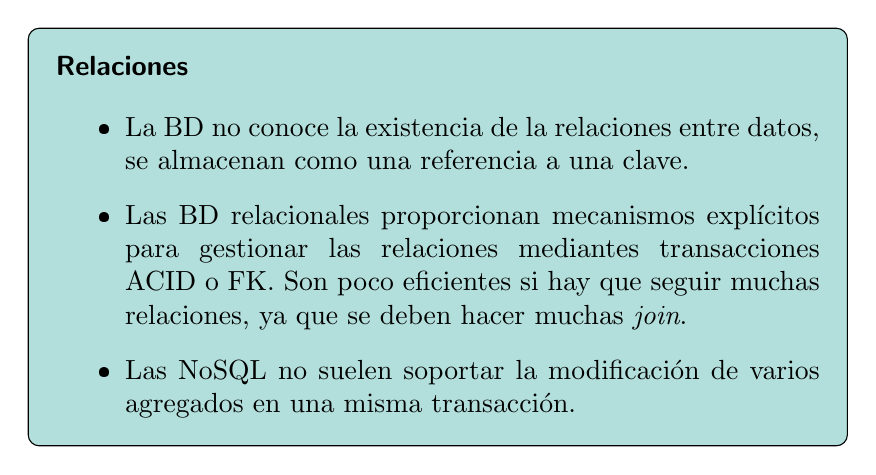
\begin{tikzpicture}
                \node[fill=mint, fill opacity=1, text opacity=1, text width=0.8\textwidth, align=justify, draw, rounded corners, inner sep=10pt] 
                (note2) at (0, 0) {
                    \textbf{\textsf{Relaciones}} \\[-10pt]
                    \begin{itemize}
                    \item La BD no conoce la existencia de la relaciones entre datos, se almacenan como una referencia a una clave.
                    \item Las BD relacionales proporcionan mecanismos explícitos para gestionar las relaciones mediantes transacciones ACID o FK. Son poco eficientes si hay que seguir muchas relaciones, ya que se deben hacer muchas \textit{join}.
                    \item Las NoSQL no suelen soportar la modificación de varios agregados en una misma transacción.
                    \end{itemize}
                };
            \end{tikzpicture}
        \end{minipage}
    };

    \node[fill=pastelpink, fill opacity=1, text opacity=1, text width=\textwidth, align=justify, draw, rounded corners, inner sep=10pt] 
    (note2) at (0, -12.1) {
        \textbf{\textsf{Trabajar sin esquema}} \\[185pt]
    };

    \node[fill=lemoncream, fill opacity=1, text opacity=1, text width=12cm, align=justify, draw, rounded corners, inner sep=10pt] 
    (note2) at (-3.3, -10.5) {
        \textbf{\textsf{Ventajas}} \\[-10pt]
        \begin{itemize}
        \item No hay que hacer asunciones a priori.
        \item Facilidad para incorporar cambios en los datos y para trabajar con datos no uniformes. 
        \item Tener esquema resulta inflexible en la inserción de datos, es común un campo de texto done va cualquier cosa.
        \end{itemize}
    };

    \node[fill=lemoncream, fill opacity=1, text opacity=1, text width=12cm, align=justify, draw, rounded corners, inner sep=10pt] 
    (note2) at (-3.3, -13.9) {
        \textbf{\textsf{Desventajas}} \\[-10pt]
        \begin{itemize}
        \item Las aplicaciones suelen necesitar cierto formato y semántica en los datos, cierto esquema implicito en los datos. Por esto, hay que minimizar el uso de literales, para que el código se pueda cambiar y mejorar de forma fácil.
        \item Tener el esquema codificado en las aplicaciones puede dar problemas, ya que la BD no puede utilizarlo para mejorar la eficiencia.
        \item Los esquemas tienen valor. Una BD sin esquema solo traslada el problema del esquema a la aplicación (es como usar un lenguaje de tipado débil). 
        \end{itemize}
    };

    \node[fill=lemoncream, fill opacity=1, text opacity=1, text width=5.75cm, align=justify, draw, rounded corners, inner sep=10pt] 
    (note2) at (6.5, -12.45) {
        \textbf{\textsf{Soluciones}} \\[-10pt]
        \begin{itemize}
        \item Integrar todo el acceso a la BD en una única app que proporciona servicios web para las demás.
        \item Delimitar diferentes partes de cada agregado para el acceso de apps diferentes.
        \end{itemize}
        Los esquemas en BD relacionales son ``flexibles'', permiten añadir y quitar columnas por ejemplo. El problema de almacenar los datos de formas nuevas en BD NoSQL es que las apps deben funcionar con datos nuevos y antiguos. Esto se puede arreglar añadiendo una columna y conviviendo con dos columnas, una con nulos hacia arriba y otra con nulos hacia abajo.
    };

    \node[fill=pastelpink, fill opacity=1, text opacity=1, text width=\textwidth, align=justify, draw, rounded corners, inner sep=10pt] 
    (note2) at (0, -20.2) {
        \textbf{\textsf{Cambios en el esquema}} \\
        Se le da importancia a los métodos ágiles para cambiar fácilmente de esquema. En NoSQL se pueden hacer cambios rápidos, pero hay que tener cuidado con las migraciones de esquema. \\[170pt]
    };

    \node[fill=lemoncream, fill opacity=1, text opacity=1, text width=0.45\textwidth, align=justify, draw, rounded corners, inner sep=10pt] 
    (note2) at (-4.95, -20) {
        \textbf{\textsf{BD relacional}} \\[-10pt]
        \begin{itemize}
        \item Un cambio de esquema puede ser un proyecto en si mismo, ya que necesita \textit{scripts} para la migración de datos.
        \item Con los proyectos nuevos simplemente almacenamos los cambios con los \textit{scripts} de migración de datos.
        \item Con proyectos \textit{legacy} extraemos el esquema de la BD y procedemos con los proyectos nuevos. Es importante mantener la compatibilidad hacia atrás y tener en cuenta que hay una fase de transición, donde ambos esquemas conviven.
        \end{itemize}
    };


    \node[fill=lemoncream, fill opacity=1, text opacity=1, text width=0.45\textwidth, align=justify, draw, rounded corners, inner sep=10pt] 
    (note2) at (5, -20.75) {
        \textbf{\textsf{BD NoSQL}} \\[-10pt]
        \begin{itemize}
        \item Se intenta no tener que realizar cambios de esquema. 
        \item El esquema está en la aplicación ! Debe \textit{parsear} los datos obtenidos de la BD, por lo que hay que cambiar el código que la app lee y escribe. Si no cambiamos la aplicación, el error de esquema que daría la BD lo dará la aplicación.
        \item Se hace una migración incremental, ya que mover todos los datos puede ser muy costoso. Transicionamos a partir e la propia aplicación, lee archivos de ambos esquemas (viejo y nuevo) pero escribe en el nuevo. De esta forma, hay datos que no llegan nunca a migrarse.
        \item En el caso de una BD de grafos, se pueden definir nuevos arcos con el nuevo esquema.
        \end{itemize}
    };

    
    

\end{tikzpicture}



\begin{tikzpicture}
    \node[fill=pastelpink, fill opacity=1, text opacity=1, text width=0.7\textwidth, align=justify, draw, rounded corners, inner sep=10pt] 
    (note1) at (0, 0) {
        \begin{minipage}{0.3\textwidth}
            \textbf{\textsf{Interés NoSQL}} \\[-10pt]
            \begin{itemize}
                \item Funciona aprovechando los recursos de un \textit{cluster} de computación
                \item Usa el agregado como unidad natural de distribución de datos.
            \end{itemize}
        \end{minipage}
        \hspace{0cm}
        \begin{minipage}{0.39\textwidth}
            \begin{tikzpicture}
                \node[fill=lemoncream, fill opacity=1, text opacity=1, text width=0.8\textwidth, align=justify, draw, rounded corners, inner sep=10pt] 
                (note2) at (0, 0) {
                    \textbf{\textsf{Ventajas}} \\[-10pt]
                    \begin{itemize}
                        \item Capacidad para gestionar un mayor volumen de datos. 
                        \item Se puede incrementar el tráfico de operaciones de lectura y escritura (rendimiento), así como la disponibilidad (tolerancia a fallos).
                    \end{itemize}
                };
            \end{tikzpicture}
        \end{minipage}
        \hspace{-0.2cm}
        \begin{minipage}{0.3\textwidth}
            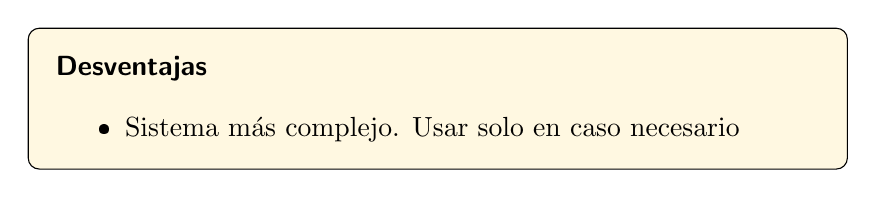
\begin{tikzpicture}
                \node[fill=lemoncream, fill opacity=1, text opacity=1, text width=0.8\textwidth, align=justify, draw, rounded corners, inner sep=10pt] 
                (note2) at (0, 0) {
                    \textbf{\textsf{Desventajas}} \\[-10pt]
                    \begin{itemize}
                        \item Sistema más complejo. Usar solo en caso necesario
                    \end{itemize}
                };
            \end{tikzpicture}
        \end{minipage}
    };

    \node[fill=powderblue, fill opacity=1, text opacity=1, text width=0.25\textwidth, align=justify, draw, rounded corners, inner sep=10pt] 
    (note1) at (10.2, 0) {
        \textbf{\textsf{Formas de replicación de los datos}} \\[-10pt]
        \begin{itemize}
        \item Replicación: se hacen varias copias del mismo dato en distintos nodos. Válida para arquitecturas maestro-esclavo o \textit{peer-to-peer}. 
        \item Particionamiento (sharding): repartir los datos entre los nodos. 
        \item Técnicas ortogonales: se pueden combinar
        \end{itemize}
    };

    \node[fill=softpeach, fill opacity=1, text opacity=1, text width=0.75\textwidth, align=justify, draw, rounded corners, inner sep=10pt] 
    (note1) at (0.45, -6.5) {
        \textbf{\textsf{Sharding}} \\[2pt]
        El particionamiento es una técnica usada cuando se tienen distintos usuarios accediendo a partes distintas de la base de datos. Para mejorar el rendimiento, se dividen los datos y se coloca cada parte en un nodo distinto. Cada \textit{shard} lee y escribe sobre su propia partición de datos. Esto nos proporciona escalabilidad horizontal.  \\

        Debemos intentar mantener la localidad de los datos, es decir, que los datos que se acceden juntos estén en el mismo nodo y cerca en el disco. Para ello, mantenemos los datos que se suelen acceder juntos en el mismo agregado y usamos el agregado como unidad de datos para la distirbución. También es recomendable mantener cerca agregados que se suelen usar juntos. \\

        Además, es recomendable mantener todos los nodos con una carga de datos similar, lo que podemos conseguir haciendo una distribución uniforme de los datos. \\

        Implementar el \textit{sharding} en el nivel de la aplicación es mucho más complejo. Muchas BD NoSQL gestionan el \textit{sharding} de forma automática. \\

        \begin{itemize}
            \item En cuanto a rendimiento, el particionamiento mejora lectura y escrituras, mientras que la replicación puede mejorar lecturas pero empeorar escrituras.
            \item En cuanto a la fiabilidad, el particionamiento no mejora la disponibilidad, aumenta la probabilidad de fallo y puede haber fallos parciales.
        \end{itemize}
    };

    \node[fill=softpeach, fill opacity=1, text opacity=1, text width=0.2\textwidth, align=justify, draw, rounded corners, inner sep=10pt] 
    (note1) at (10.7, -5) {
        \textbf{\textsf{Un solo servidor}} \\[2pt]
        En este caso no existe la distribución de datos. Es la opción preferida por ser el mas simple, y el uso de NoSQL se justificaría por cuestiones relacionadas con el modelo de datos. Las BD de grafos suelen usar esta arquitectura. Los datos agregados se procesan en el nivel de la aplicación y se recuperan juntos.
    };

    \node[fill=softpeach, fill opacity=1, text opacity=1, text width=0.75\textwidth, align=justify, draw, rounded corners, inner sep=10pt] 
    (note1) at (0.45, -14) {
        \begin{minipage}{0.39\textwidth}
            \textbf{\textsf{Replicación Maestro-Esclavo}} \\[-10pt]
            \begin{itemize}
            \item Buena solución cuando la aplicación es intensiva en lecturas. Aquí, los datos se reparte en varios nodos.
            \item Un nodo es elegido como maestro (autoridad como fuente de los datos y responsable de su actualización) y el resto son esclavos.
            \item El proceso de replicación sincroniza los esclavos con el maestro. Cuanto más síncrono, mayor consistencia pero menos rendimiento y disponibilidad.
            \end{itemize}
            
        \end{minipage}
        \hspace{0cm}
        \begin{minipage}{0.3\textwidth}
            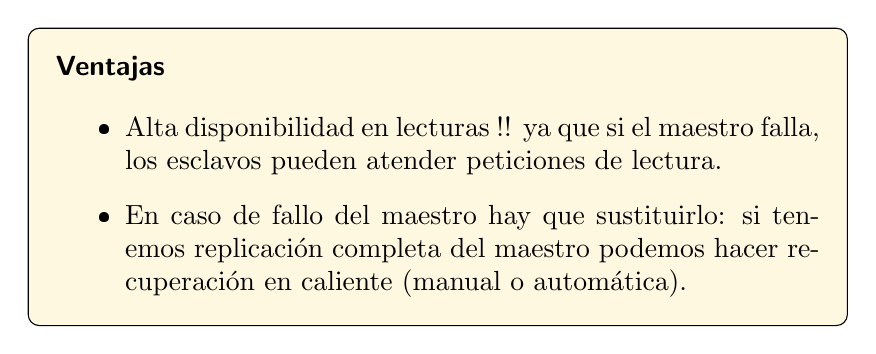
\begin{tikzpicture}
                \node[fill=lemoncream, fill opacity=1, text opacity=1, text width=0.8\textwidth, align=justify, draw, rounded corners, inner sep=10pt] 
                (note2) at (0, 0) {
                    \textbf{\textsf{Ventajas}} \\[-10pt]
                    \begin{itemize}
                        \item Alta disponibilidad en lecturas !! ya que si el maestro falla, los esclavos pueden atender peticiones de lectura.
                        \item En caso de fallo del maestro hay que sustituirlo: si tenemos replicación completa del maestro podemos hacer recuperación en
                        caliente (manual o automática).
                    \end{itemize}
                };
            \end{tikzpicture}
        \end{minipage}
        \hspace{-0.2cm}
        \begin{minipage}{0.3\textwidth}
            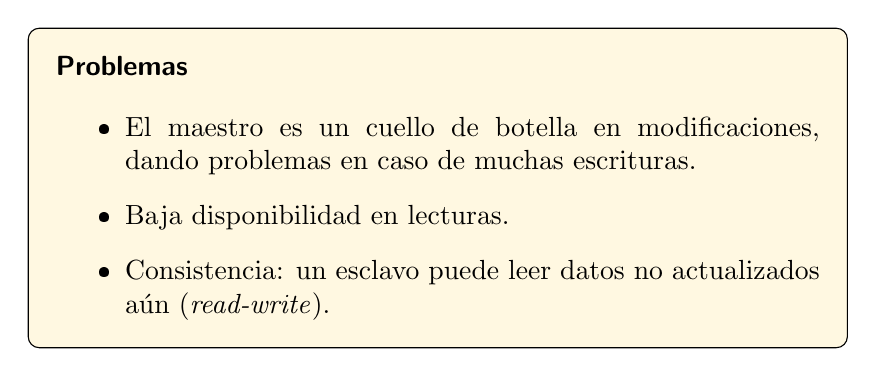
\begin{tikzpicture}
                \node[fill=lemoncream, fill opacity=1, text opacity=1, text width=0.8\textwidth, align=justify, draw, rounded corners, inner sep=10pt] 
                (note2) at (0, 0) {
                    \textbf{\textsf{Problemas}} \\[-10pt]
                    \begin{itemize}
                        \item El maestro es un cuello de botella en modificaciones, dando problemas en caso de muchas escrituras. 
                        \item Baja disponibilidad en lecturas.
                        \item Consistencia: un esclavo puede leer datos no actualizados aún (\textit{read-write}).
                    \end{itemize}
                };
            \end{tikzpicture}
        \end{minipage}
    };

    \node[fill=softpeach, fill opacity=1, text opacity=1, text width=\textwidth, align=justify, draw, rounded corners, inner sep=10pt] 
    (note1) at (2.87, -20.2) {
        \begin{minipage}{0.4\textwidth}
            \textbf{\textsf{Replicación \textit{Peer-to-peer}}} \\[-10pt]
            \begin{itemize}
            \item Motivada por los problemas de la replicación maestro-esclavo: escalabilidad en escritura y baja disponibilidad, el maestro es cuello de botella y punto único de fallo.
            \item Ahora, se elimina la distinción entre maestro y esclavo, todos los nodos se comunican entre ellos y pueden leer y escribir todos los datos.
            \end{itemize}
            
        \end{minipage}
        \hspace{0cm}
        \begin{minipage}{0.3\textwidth}
            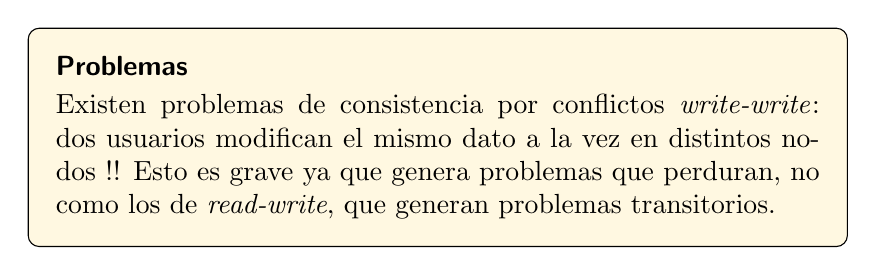
\begin{tikzpicture}
                \node[fill=lemoncream, fill opacity=1, text opacity=1, text width=0.8\textwidth, align=justify, draw, rounded corners, inner sep=10pt] 
                (note2) at (0, 0) {
                    \textbf{\textsf{Problemas}} \\[2pt]
                    Existen problemas de consistencia por conflictos \textit{write-write}: dos usuarios modifican el mismo dato a la vez en distintos nodos !! Esto es grave ya que genera problemas que perduran, no como los de \textit{read-write}, que generan problemas transitorios. 
                };
            \end{tikzpicture}
        \end{minipage}
        \hspace{-0.2cm}
        \begin{minipage}{0.3\textwidth}
            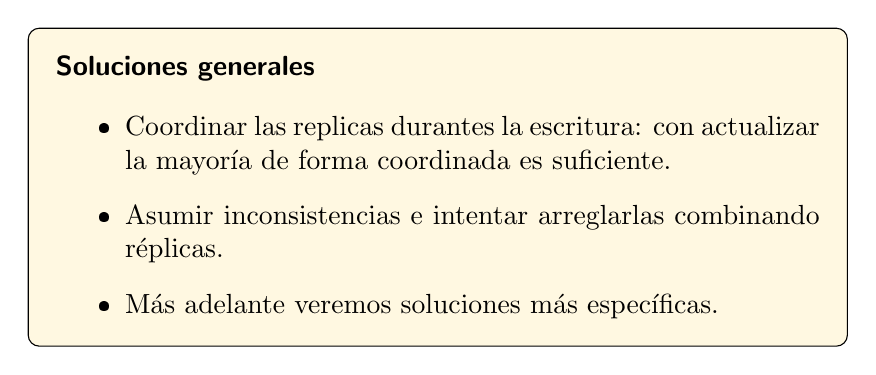
\begin{tikzpicture}
                \node[fill=lemoncream, fill opacity=1, text opacity=1, text width=0.8\textwidth, align=justify, draw, rounded corners, inner sep=10pt] 
                (note2) at (0, 0) {
                    \textbf{\textsf{Soluciones generales}} \\[-10pt]
                    \begin{itemize}
                        \item Coordinar las replicas durantes la escritura: con actualizar la mayoría de forma coordinada es suficiente.
                        \item Asumir inconsistencias e intentar arreglarlas combinando réplicas.
                        \item Más adelante veremos soluciones más específicas.
                    \end{itemize}
                };
            \end{tikzpicture}
        \end{minipage}
    };

    \node[fill=powderblue, fill opacity=1, text opacity=1, text width=0.2\textwidth, align=justify, draw, rounded corners, inner sep=10pt] 
    (note1) at (10.7, -11.7) {
        \textbf{\textsf{Combinación particionamiento-replicación}} \\[2pt]
        \begin{itemize}
        \item Con maestro-esclavo: usariamos un maestro para cada partición. Dependiendo de la configuración, podemos elegir maestro y esclavos a nivel \textit{cluster} o para cada partición.
        \item Con \textit{peer-to-peer}: común en NoSQL con modelos de tipo \textit{column-family}. Se usa una replicación con factor 3, por lo que cada partición tiene 3 copias en 3 nodos y si un nodo falla, sus particiones se distribuyen entre los demás.
        \end{itemize}
    };

\end{tikzpicture}




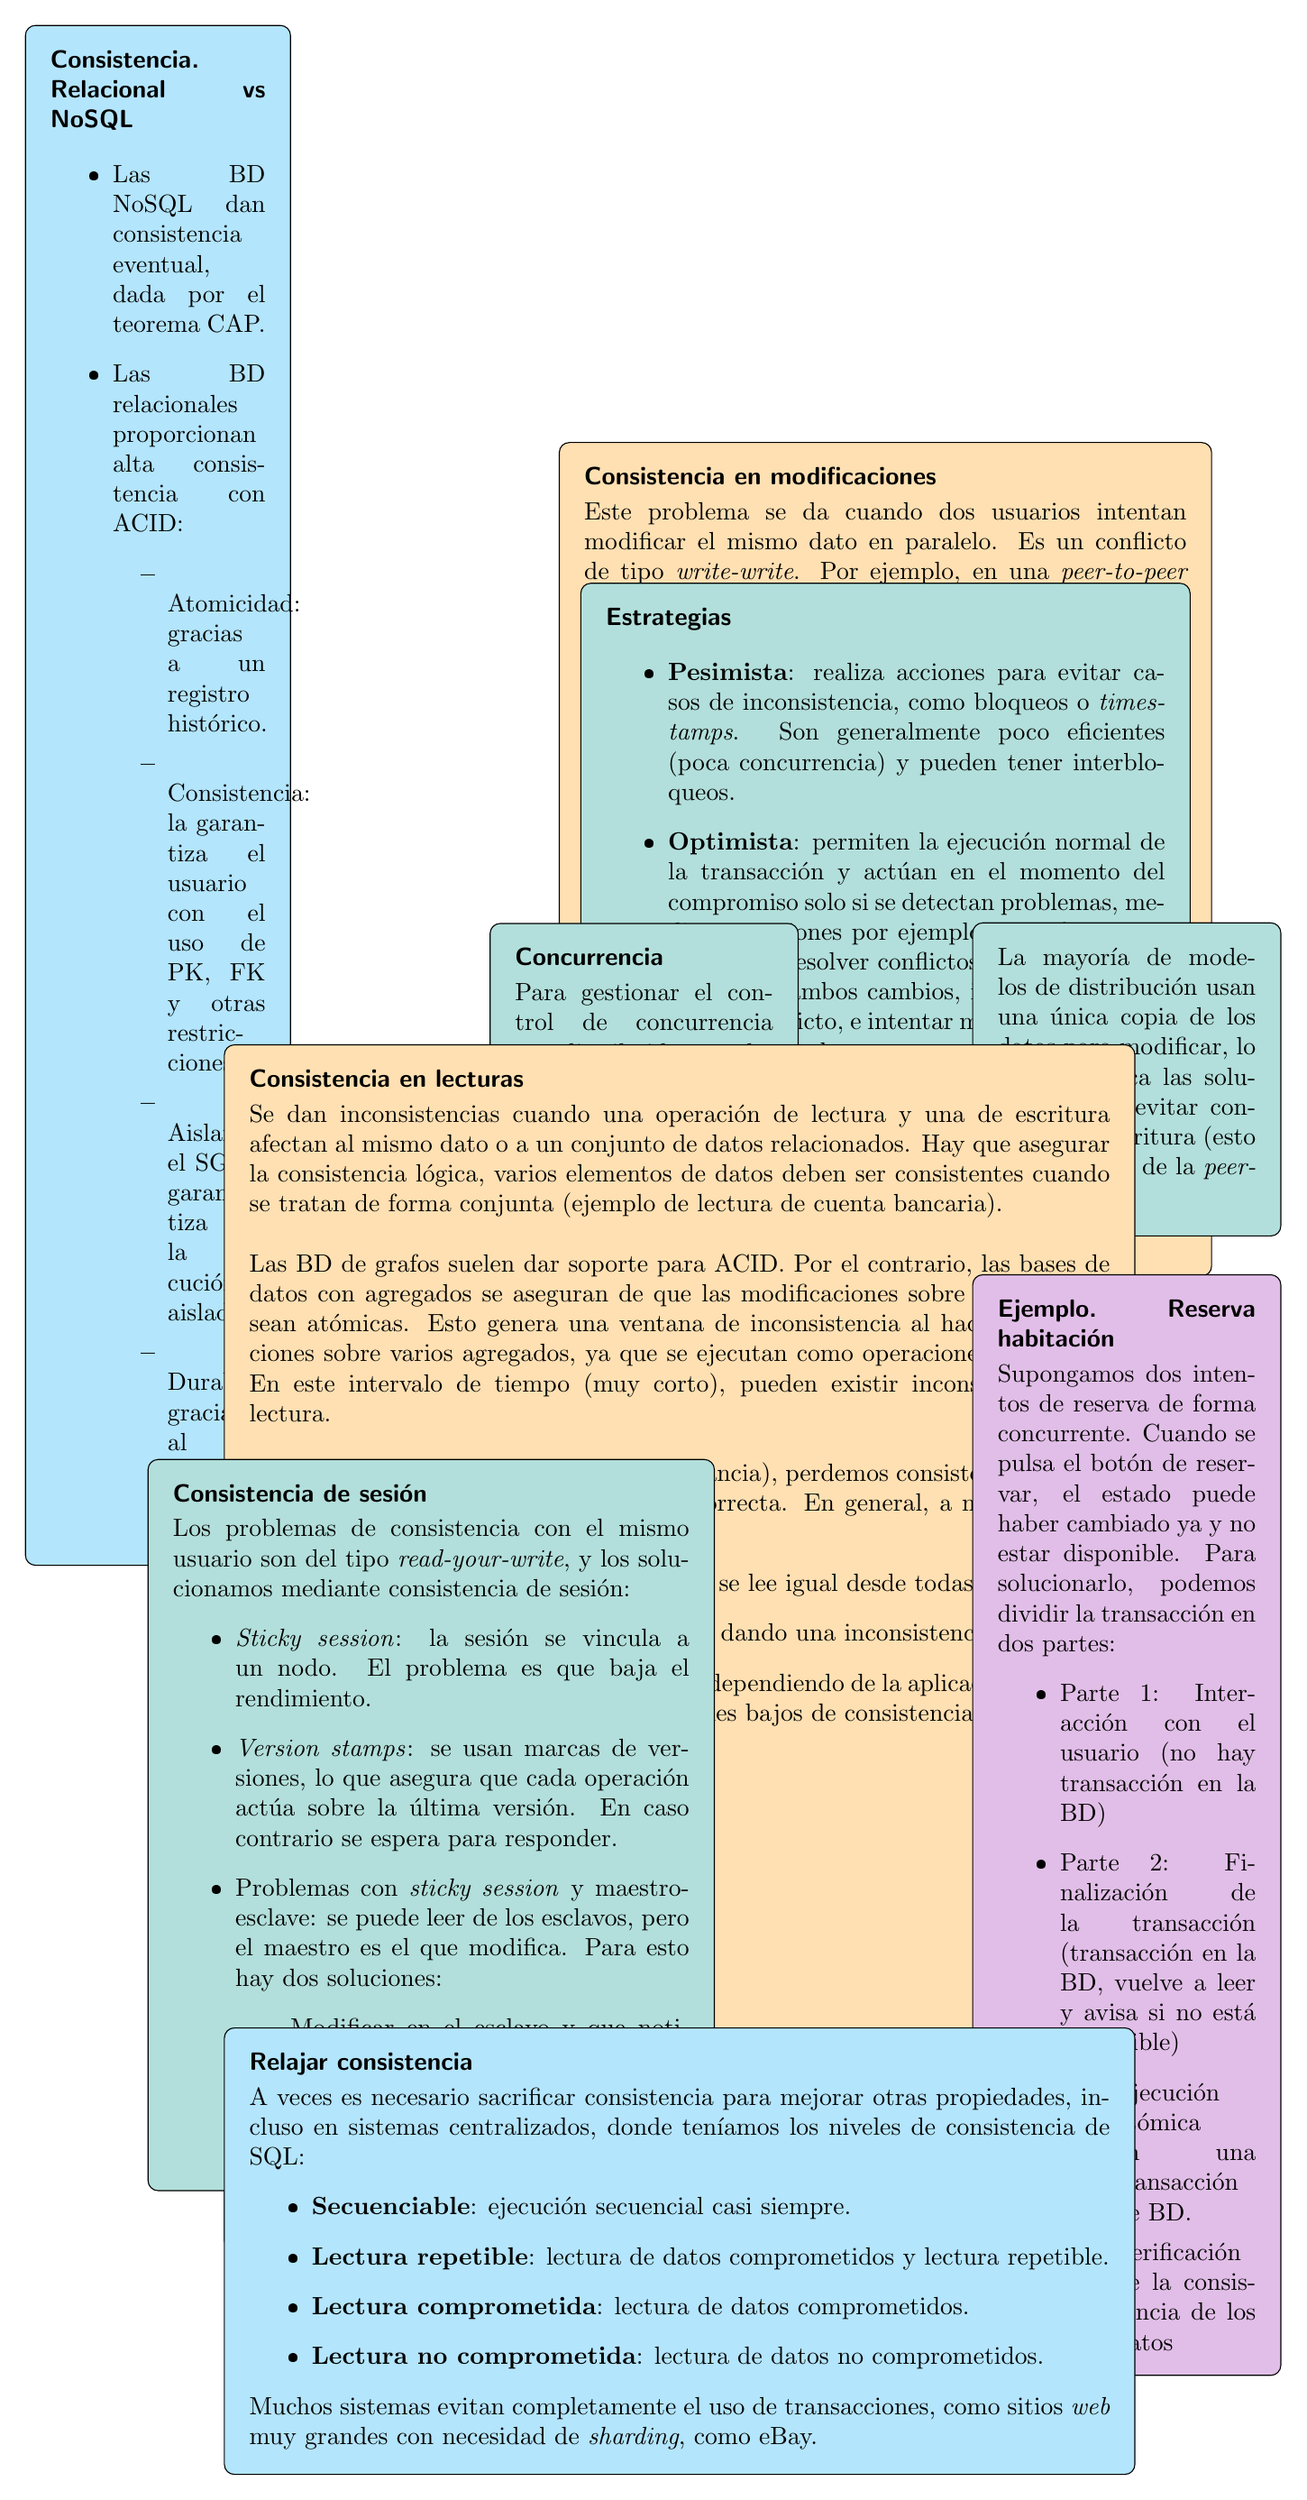
\begin{tikzpicture}
    \node[fill=powderblue, fill opacity=1, text opacity=1, text width=0.25\textwidth, align=justify, draw, rounded corners, inner sep=10pt] 
    (note1) at (-3.85, 0) {
        \textbf{\textsf{Consistencia. Relacional vs NoSQL}} \\[-10pt]
        \begin{itemize}
        \item Las BD NoSQL dan consistencia eventual, dada por el teorema CAP.
        \item Las BD relacionales proporcionan alta consistencia con ACID:
        \begin{itemize}
        \item Atomicidad: gracias a un registro histórico.
        \item Consistencia: la garantiza el usuario con el uso de PK, FK y otras restricciones.
        \item Aislamiento: el SGBD garantiza la ejecución aislada.
        \item Durabilidad: gracias al registro histórico y copias.
        \end{itemize}
        \end{itemize}
    };

    \node[fill=softpeach, fill opacity=1, text opacity=1, text width=0.7\textwidth, align=justify, draw, rounded corners, inner sep=10pt] 
    (note1) at (6.4, -0.9) {
        \textbf{\textsf{Consistencia en modificaciones}} \\[2pt]
        Este problema se da cuando dos usuarios intentan modificar el mismo dato en paralelo. Es un conflicto de tipo \textit{write-write}. Por ejemplo, en una \textit{peer-to-peer} dos replicas pueden aplicar las mismas modificaciones en distinto orden: uno lee, modifica y escribe, y otro modifica entre que el primero lee y modifica. El primero escribe y luego el segundo escribe. DEBE HABER UN COMPROMISO ENTRE CONSISTENCIA Y EFICIENCIA. \\ [185pt]
    };

    \node[fill=mint, fill opacity=1, text opacity=1, text width=0.65\textwidth, align=justify, draw, rounded corners, inner sep=10pt] 
    (note1) at (6.4, -0.8) {
        \textbf{\textsf{Estrategias}} \\[-10pt]
        \begin{itemize}
        \item \textbf{Pesimista}: realiza acciones para evitar casos de inconsistencia, como bloqueos o \textit{timestamps}. Son generalmente poco eficientes (poca concurrencia) y pueden tener interbloqueos.
        \item \textbf{Optimista}: permiten la ejecución normal de la transacción y actúan en el momento del compromiso solo si se detectan problemas, mediante versiones por ejemplo. Una forma optimista de resolver conflictos \textit{write-write} sería almacenar ambos cambios, indicando que existe un conflicto, e intentar mezclar ambas versiones para obtener una versión consistente (complicado).
        \end{itemize}
    };

    \node[fill=mint, fill opacity=1, text opacity=1, text width=0.3\textwidth, align=justify, draw, rounded corners, inner sep=10pt] 
    (note1) at (3, -4) {
        \textbf{\textsf{Concurrencia}} \\[2pt]
        Para gestionar el control de concurrencia en distribuido, podemos dar consistencia secuencial, aplicando las operaciones en el mismo orden en todos los nodos.
    };

    \node[fill=mint, fill opacity=1, text opacity=1, text width=0.3\textwidth, align=justify, draw, rounded corners, inner sep=10pt] 
    (note1) at (9.8, -4) {
        La mayoría de modelos de distribución usan una única copia de los datos para modificar, lo que simplifica las soluciones para evitar conflictos de escritura (esto no es el caso de la \textit{peer-to-peer}).
    };

    \node[fill=softpeach, fill opacity=1, text opacity=1, text width=\textwidth, align=justify, draw, rounded corners, inner sep=10pt] 
    (note1) at (3.5, -12) {
        \textbf{\textsf{Consistencia en lecturas}} \\[2pt]
        Se dan inconsistencias cuando una operación de lectura y una de escritura afectan al mismo dato o a un conjunto de datos relacionados. Hay que asegurar la consistencia lógica, varios elementos de datos deben ser consistentes cuando se tratan de forma conjunta (ejemplo de lectura de cuenta bancaria). \\

        Las BD de grafos suelen dar soporte para ACID. Por el contrario, las bases de datos con agregados se aseguran de que las modificaciones sobre un agregado sean atómicas. Esto genera una ventana de inconsistencia al hacer modificaciones sobre varios agregados, ya que se ejecutan como operaciones separadas. En este intervalo de tiempo (muy corto), pueden existir inconsistencias en lectura. \\

        Al introducir replicacion (y añadir redundancia), perdemos consistencia, ya que hay que gestionar las réplicas de forma correcta. En general, a mayor redundancia, menor consistencia
        \begin{itemize}
        \item Hay que asegurar que el mismo dato se lee igual desde todas las réplicas. 
        \item Un problema de lectura es temporal, dando una inconsistencia eventual. 
        \item El nivel de consistencia lo ajustamos dependiendo de la aplicación; muchas operaciones pueden hacerse con niveles bajos de consistencia. 
        \end{itemize} 
        \quad \\[170pt]
    };

    \node[fill=mint, fill opacity=1, text opacity=1, text width=0.6\textwidth, align=justify, draw, rounded corners, inner sep=10pt] 
    (note1) at (0, -14.5) {
        \textbf{\textsf{Consistencia de sesión}} \\[2pt]
        Los problemas de consistencia con el mismo usuario son del tipo \textit{read-your-write}, y los solucionamos mediante consistencia de sesión:
        \begin{itemize}
        \item \textit{Sticky session}: la sesión se vincula a un nodo. El problema es que baja el rendimiento.
        \item \textit{Version stamps}: se usan marcas de versiones, lo que asegura que cada operación actúa sobre la última versión. En caso contrario se espera para responder.
        \item Problemas con \textit{sticky session} y maestro-esclave: se puede leer de los esclavos, pero el maestro es el que modifica. Para esto hay dos soluciones:
        \begin{itemize}
        \item Modificar en el esclavo y que notifique al maestro.
        \item Mover la sesión al maestro mientras se realiza la modificación y, al actualizar cambios, volver al esclavo.
        \end{itemize}
        \end{itemize}
    };

    \node[fill=lavender, fill opacity=1, text opacity=1, text width=0.3\textwidth, align=justify, draw, rounded corners, inner sep=10pt] 
    (note1) at (9.8, -14.5) {
        \textbf{\textsf{Ejemplo. Reserva habitación}} \\[2pt]
        Supongamos dos intentos de reserva de forma concurrente. Cuando se pulsa el botón de reservar, el estado puede haber cambiado ya y no estar disponible. Para solucionarlo, podemos dividir la transacción en dos partes:
        \begin{itemize}
        \item Parte 1: Interacción con el usuario (no hay transacción en la BD)
        \item Parte 2: Finalización de la transacción (transacción en la BD, vuelve a leer y avisa si no está disponible)
        \begin{itemize}
        \item Ejecución atómica en una transacción de BD.
        \item Verificación de la consistencia de los datos
        \end{itemize}
        \end{itemize}
    };

    \node[fill=powderblue, fill opacity=1, text opacity=1, text width=\textwidth, align=justify, draw, rounded corners, inner sep=10pt] 
    (note1) at (3.5, -20.5) {
        \textbf{\textsf{Relajar consistencia}} \\[2pt]
        A veces es necesario sacrificar consistencia para mejorar otras propiedades, incluso en sistemas centralizados, donde teníamos los niveles de consistencia de SQL:
        \begin{itemize}
        \item \textbf{Secuenciable}: ejecución secuencial casi siempre.
        \item \textbf{Lectura repetible}: lectura de datos comprometidos y lectura repetible.
        \item \textbf{Lectura comprometida}: lectura de datos comprometidos.
        \item \textbf{Lectura no comprometida}: lectura de datos no comprometidos.
        \end{itemize}
        Muchos sistemas evitan completamente el uso de transacciones, como sitios \textit{web} muy grandes con necesidad de \textit{sharding}, como eBay.
    };

\end{tikzpicture}


\newpage















































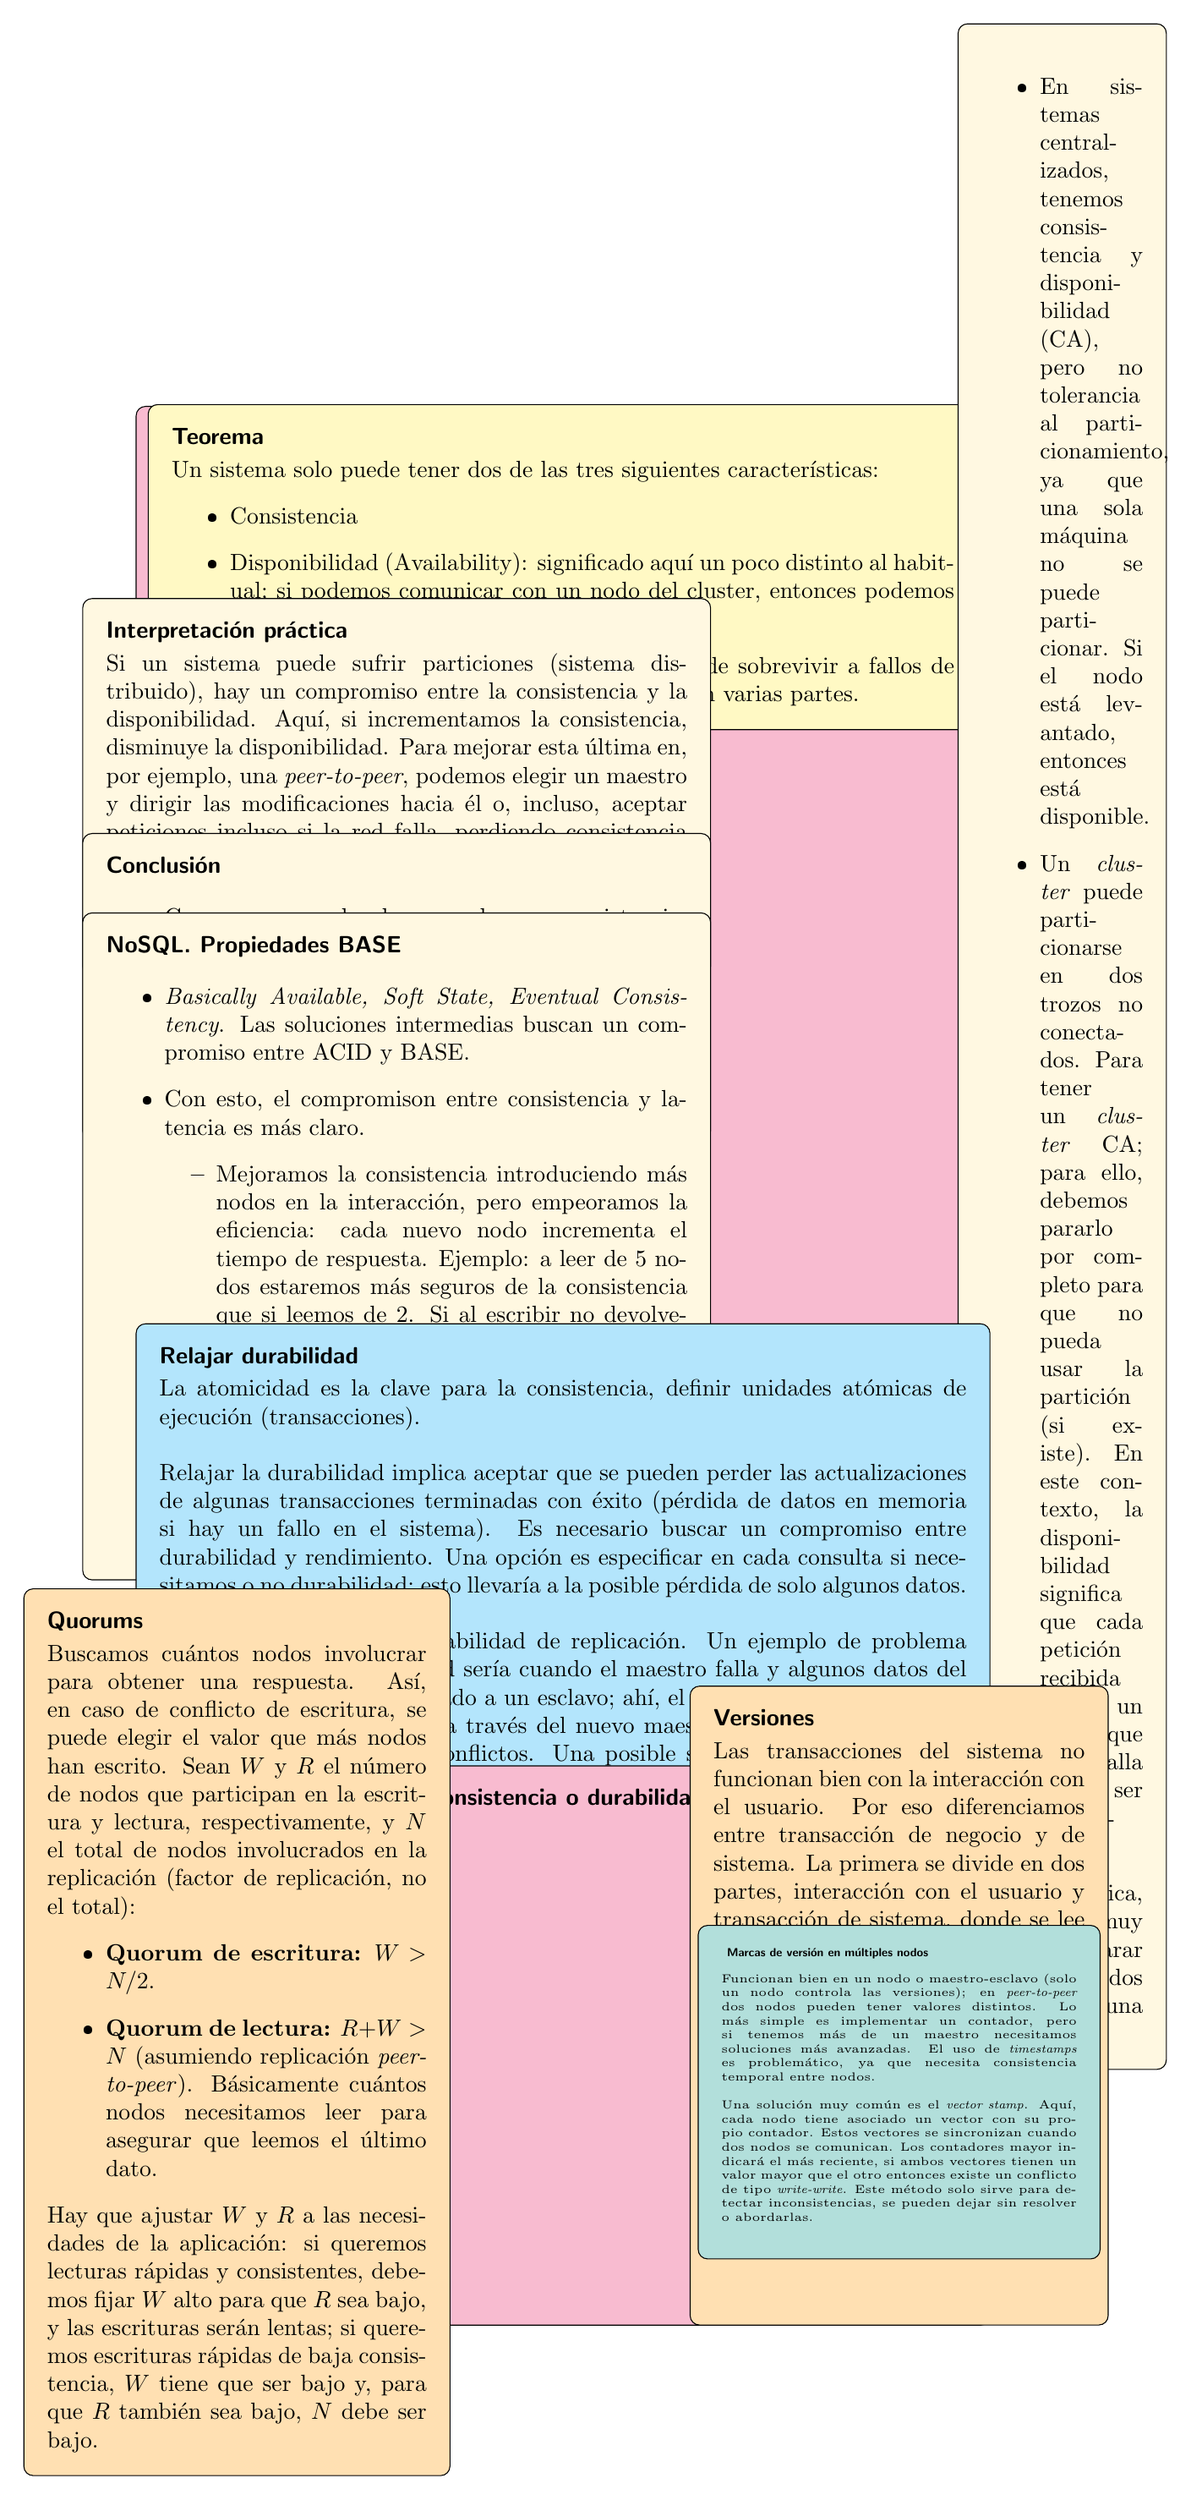
\begin{tikzpicture}

    \node[fill=pastelpink, fill opacity=1, text opacity=1, text width=\textwidth, align=justify, draw, rounded corners, inner sep=10pt] 
    (note1) at (3.5, -20.5) {
        \textbf{\textsf{Teorema CAP}} \\[400pt]
    };

    \node[fill=lightyellow, fill opacity=1, text opacity=1, text width=0.97\textwidth, align=justify, draw, rounded corners, inner sep=10pt] 
    (note1) at (3.5, -15.2) {
        \textbf{\textsf{Teorema}} \\[2pt]
        Un sistema solo puede tener dos de las tres siguientes características:
        \begin{itemize}
        \item Consistencia
        \item Disponibilidad (Availability): significado aquí un poco distinto al habitual; si podemos comunicar con un nodo del cluster, entonces podemos leer y escribir datos.
        \item Tolerancia al particionamiento: el cluster puede sobrevivir a fallos de comunicación entre los nodos que lo separan en varias partes.
        \end{itemize}
    };

    \node[fill=lemoncream, fill opacity=1, text opacity=1, text width=0.2\textwidth, align=justify, draw, rounded corners, inner sep=10pt] 
    (note1) at (11, -22.4) {
        \begin{itemize}
        \item En sistemas centralizados, tenemos consistencia y disponibilidad (CA), pero no tolerancia al particionamiento, ya que una sola máquina no se puede particionar. Si el nodo está levantado, entonces está disponible. 
        \item Un \textit{cluster} puede particionarse en dos trozos no conectados. Para tener un \textit{cluster} CA; para ello, debemos pararlo por completo para que no pueda usar la partición (si existe). En este contexto, la disponibilidad significa que cada petición recibida por un nodo que no falla debe ser respondida.
        \end{itemize}
        En la práctica, resulta muy costoso parar todos los nodos cuando hay una partición. 
    };

    \node[fill=lemoncream, fill opacity=1, text opacity=1, text width=0.72\textwidth, align=justify, draw, rounded corners, inner sep=10pt] 
    (note1) at (1, -18.5) {
        \textbf{\textsf{Interpretación práctica}} \\[2pt]
        Si un sistema puede sufrir particiones (sistema distribuido), hay un compromiso entre la consistencia y la disponibilidad. Aquí, si incrementamos la consistencia, disminuye la disponibilidad. Para mejorar esta última en, por ejemplo, una \textit{peer-to-peer}, podemos elegir un maestro y dirigir las modificaciones hacia él o, incluso, aceptar peticiones incluso si la red falla, perdiendo consistencia (en el caso de la reserva de habitación, tendríamos \textit{overbooking}). Otro ejemplo sería el carro de la compra de Amazon, que escribe todos los carros aunque falle y luego une. 
    };

    \node[fill=lemoncream, fill opacity=1, text opacity=1, text width=0.72\textwidth, align=justify, draw, rounded corners, inner sep=10pt] 
    (note1) at (1, -21.5) {
        \textbf{\textsf{Conclusión}} \\[-10pt]
        \begin{itemize}
        \item Como programador hay que buscar consistencia, pero se puede relajar para conseguir disponibilidad y mejorar eficiencia.
        \item La consistencia de lectura es importante, junto con la duración de la ventana de inconsistencia y la toleracia a lecturas viejas. El último dato es de gran importancia.
        \end{itemize} 
    };

    \node[fill=lemoncream, fill opacity=1, text opacity=1, text width=0.72\textwidth, align=justify, draw, rounded corners, inner sep=10pt] 
    (note1) at (1, -25.4) {
        \textbf{\textsf{NoSQL. Propiedades BASE}} \\[-10pt]
        \begin{itemize}
        \item \textit{Basically Available, Soft State, Eventual Consistency}. Las soluciones intermedias buscan un compromiso entre ACID y BASE.
        \item Con esto, el compromison entre consistencia y latencia es más claro.
        \begin{itemize}
        \item Mejoramos la consistencia introduciendo más nodos en la interacción, pero empeoramos la eficiencia: cada nuevo nodo incrementa el tiempo de respuesta. Ejemplo: a leer de 5 nodos estaremos más seguros de la consistencia que si leemos de 2. Si al escribir no devolvemos el control hasta que 5 nodos hayan escrito, tendremos más consistencia que si esperamos por 2.
        \item La disponibilidad es el límite de la latencia que podemos tolerar en la aplicación. Aquí relacionamos disponibilidad con eficiencia: cuando la latencia es muy alta, nos rendimos y asumimos que la operación no puede terminar.
        \end{itemize}
        \end{itemize} 
    };

    \node[fill=powderblue, fill opacity=1, text opacity=1, text width=\textwidth, align=justify, draw, rounded corners, inner sep=10pt] 
    (note1) at (3.5, -30.7) {
        \textbf{\textsf{Relajar durabilidad}} \\[2pt]
        La atomicidad es la clave para la consistencia, definir unidades atómicas de ejecución (transacciones). \\
        
        Relajar la durabilidad implica aceptar que se pueden perder las actualizaciones de algunas transacciones terminadas con éxito (pérdida de datos en memoria si hay un fallo en el sistema). Es necesario buscar un compromiso entre durabilidad y rendimiento. Una opción es especificar en cada consulta si necesitamos o no durabilidad; esto llevaría a la posible pérdida de solo algunos datos. \\

        Otro factor clave es la durabilidad de replicación. Un ejemplo de problema por falta de esta durabilidad sería cuando el maestro falla y algunos datos del maestro no se habían replicado a un esclavo; ahí, el esclavo busca otro maestro y sigue recibiendo cambios a través del nuevo
        maestro. Si el maestro antiguo se recupera, puede haber conflictos. Una posible solución es esperar a tener las réplicas generadas para comprometer la transacción, lo que mejora la durabilidad de replicación, empeora el rendimiento de las escrituras y disminuye la disponibilidad (aumenta la probabilidad de fallo de la escritura).
    };

    \node[fill=pastelpink, fill opacity=1, text opacity=1, text width=\textwidth, align=justify, draw, rounded corners, inner sep=10pt] 
    (note1) at (3.5, -37.4) {
        \textbf{\textsf{Soluciones reales para la consistencia o durabilidad}} \\[200pt]
    };

    \node[fill=softpeach, fill opacity=1, text opacity=1, text width=0.47\textwidth, align=justify, draw, rounded corners, inner sep=10pt] 
    (note1) at (-1.4, -37.2) {
        \textbf{\textsf{Quorums}} \\[2pt]
        Buscamos cuántos nodos involucrar para obtener una respuesta. Así, en caso de conflicto de escritura, se puede elegir el valor que más nodos han escrito. Sean $W$ y $R$ el número de nodos que participan en la escritura y lectura, respectivamente, y $N$ el total de nodos involucrados en la replicación (factor de replicación, no el total):
        \begin{itemize}
        \item \textbf{Quorum de escritura:}  $W > N/2$.
        \item \textbf{Quorum de lectura:} $R + W > N$ (asumiendo replicación \textit{peer-to-peer}). Básicamente cuántos nodos necesitamos leer para asegurar que leemos el último dato.
        \end{itemize}
        Hay que ajustar $W$ y $R$ a las necesidades de la aplicación: si queremos lecturas rápidas y consistentes, debemos fijar $W$ alto para que $R$ sea bajo, y las escrituras serán lentas; si queremos escrituras rápidas de baja consistencia, $W$ tiene que ser bajo y, para que $R$ también sea bajo, $N$ debe ser bajo.
    };

    \node[fill=softpeach, fill opacity=1, text opacity=1, text width=0.46\textwidth, align=justify, draw, rounded corners, inner sep=10pt] 
    (note1) at (8.55, -36.8) {
        \textbf{\textsf{Versiones}} \\[2pt]
        Las transacciones del sistema no funcionan bien con la interacción con el usuario. Por eso diferenciamos entre transacción de negocio y de sistema. La primera se divide en dos partes, interacción con el usuario y transacción de sistema, donde se lee todo de nuevo para comprobar si ha cambiado (se hace por medio de marcas de versión, como contadores, \textit{timestamps} o \textit{hash} de elementos). \\[100pt]
    };

    \node[fill=mint, fill opacity=1, text opacity=1, text width=0.44\textwidth, align=justify, draw, rounded corners, inner sep=10pt] 
    (note1) at (8.55, -38.1) {
        \begin{tiny}
        \textbf{\textsf{Marcas de versión en múltiples nodos}} \\[-1pt]
        \begin{spacing}{1}
        Funcionan bien en un nodo o maestro-esclavo (solo un nodo controla las versiones); en \textit{peer-to-peer} dos nodos pueden tener valores distintos. Lo más simple es implementar un contador, pero si tenemos más de un maestro necesitamos soluciones más avanzadas. El uso de \textit{timestamps} es problemático, ya que necesita consistencia temporal entre nodos. \\

        Una solución muy común es el \textit{vector stamp}. Aquí, cada nodo tiene asociado un vector con su propio contador. Estos vectores se sincronizan cuando dos nodos se comunican. Los contadores mayor indicará el más reciente, si ambos vectores tienen un valor mayor que el otro entonces existe un conflicto de tipo \textit{write-write}. Este método solo sirve para detectar inconsistencias, se pueden dejar sin resolver o abordarlas.
        \end{spacing}
        \end{tiny}
    };
\end{tikzpicture}

\end{footnotesize}

\end{document}
